\documentclass[12pt]{article}

\usepackage[a4paper, left=3cm, right=2.5cm]{geometry}
\usepackage[utf8]{inputenc}
\usepackage[english]{babel}
\usepackage{blindtext}
\usepackage{microtype}
\usepackage{graphicx}
\usepackage{float}
\usepackage{wrapfig}
\usepackage{amsmath}
\usepackage[absolute]{textpos}
\usepackage{calc}
\usepackage{hyperref}
\usepackage{listings}
\usepackage{csquotes}

\setcounter{secnumdepth}{4}
\renewcommand{\baselinestretch}{1.2}


\author{Christoph Prenissl}
\date{\today}

\begin{document}

\begin{titlepage}

      \begin{textblock*}{200mm}(4mm, 10mm)
            \begin{figure}
                  \def\svgscale{0.6}
                  \input{oth_logo.pdf_tex}
            \end{figure}
      \end{textblock*}

      \begin{textblock*}{200mm}(96mm, 10mm)
            \begin{tabular}[h]{lr}
                  \textbf{Name:}       & Christoph Prenissl                                                                              \\
                  \textbf{Email:}      & \href{mailto:christoph.prenissl@st.oth-regensburg.de}{christoph.prenissl@st.oth-regensburg.de}\ \\
                  \textbf{Student ID:} & 3174997                                                                                         \\
            \end{tabular}
      \end{textblock*}

      \begin{flushright}
            \today
      \end{flushright}

      \vspace{2cm}

      \begin{center}
            \textbf{\Large{IMDB Software to fetch data of Hollywood Actors and Actresses}}

            \vspace{6cm}

            \textbf{Task 4 Document - Project Report}

            \vspace{10cm}
      \end{center}
\end{titlepage}

\newpage

\tableofcontents

\newpage

\section{Project Description}
This project mainly consists of creating a Python client to fetch data of the 
\textit{IMDB Top 50 Actors and Actresseslist} and also gather their movie data. 
The client uses an API to fetch all the basic actors/actresses list (\ref{list-actors}),
the actor/actress About section (\ref{about}) and all their movies (\ref{movies}).
For Sections \ref{awards} - \ref{top-movies} Web-scraping is used to 
get awards data and ratings of the movies.
The client is presented in a window based UserInterface where the user 
can click to gather the wanted information.

The further details of the specifics are handled in this document.

\section{Tools, Modules and Data-Structure}
\subsection{Presentation Tools}
For presenting the project I also used VS Code. I wrote the reports in \textit{\LaTeX} with the help of the \textit{LaTex Workshop} extension and 
\textit{PlantUml} to present core structures and flows of the client.
In the presentation of the client I used \textit{Powerpoint}. 

\subsection{Development Tools}
For development of the client I used \textit{Python 3.9.4} in \textit{Visual Studio 
Code} with the \textit{Python IntelliSense} extension which helped me in code 
completion and understanding the structure of all the frameworks and modules. For 
version control I used \textit{Git} and the helpful VS Code extension 
\textit{GitLens} which helped me to keep track of my changes in the project files.

The UI was designed with \textit{Qt Designer}. It was very convenient to
have a graphical UserInterface to drag and drop widgets and have an overal 
understanding of all elements.

\subsection{Modules}
When it comes to the modules, \textit{Requests} and \textit{BeautifulSoup 4} were  
necessary to handle all the web scraping. The http context is created with the 
module \textit{SSL}. For most data I used a data frame created with \textit{Pandas}.

The Graphical UserInterface was implemented using \textit{PyQt6}. The framework also
provides Thread libraries to help with multi-threading.

\section{Design}
The client has one base module at the root of the project and the children modules 
\textit{landing} and \textit{detail}.

\begin{figure}[H]
      \begin{center}
            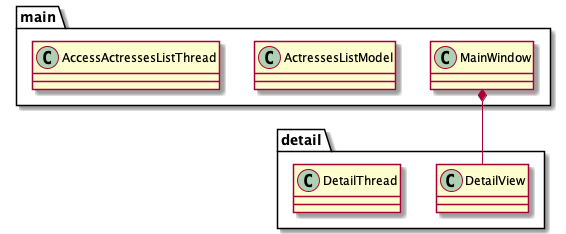
\includegraphics[scale=0.32]{img/class_diagram.png}
            \caption{\label{fig:packages} All packages used in the project with
                  the most important classes.}
      \end{center}
\end{figure}

While the base module only contains the entry point in the \textit{main.py} file,

the \textit{landing} module handles the asynchronous fetching of the actresses 
list (\ref{list-actors}), visualisation and interaction with the list and initializes an DetailView 
from \textit{detail} when a list element gets accessed.
\textit{MainWindow} is a QObject class which handles the UI update and communicates with 
\textit{AccessActressesListThread} for data provision. For the ListView containing the actresses/actors 
in MainWindow \textit{ActressesListModel} is used for correctly displaying the actor/actress data.
\textit{ActressListElement} is a data wrapper for all the data to present in the list.

The \textit{detail} module helds logic for fetching deeper information with multi-threading on 
an actor or actress regarding ratings and awards. It also contains the code for UI displaying and 
updates.
The \textit{DetailView} class acts analogously to MainView as an controller for handling UI updates and
triggering events on its threads. These threads manage the workers \textit{MoviesDataWorker} and 
\textit{ActressAwardDataWorker} for retrieving the needed data. \textit{ActressDetail} functions as a 
wrapper for a data instance.

\section{Functionalities}
\subsection{List of all available actors and actresses} \label{list-actors}

\subsection{About the actor/actresses} \label{about}

\subsection{All time movie names and years} \label{movies}

\subsection{Awards to actor/actresses in different years} \label{awards}

\subsection{Movie genre of actor/actresses} \label{genre}

\subsection{Average rating of their movies} \label{average-rating}

\subsection{Top 5 movies, their respective years and genre} \label{top-movies}

\end{document}
